%!TEX root = informe.tex
\setcounter{chapter}{1}
\addcontentsline{toc}{chapter}{\protect\numberline{\thechapter}Plano modelo adoquín Holanda 6}

\begin{figure}[!htb]
\centering
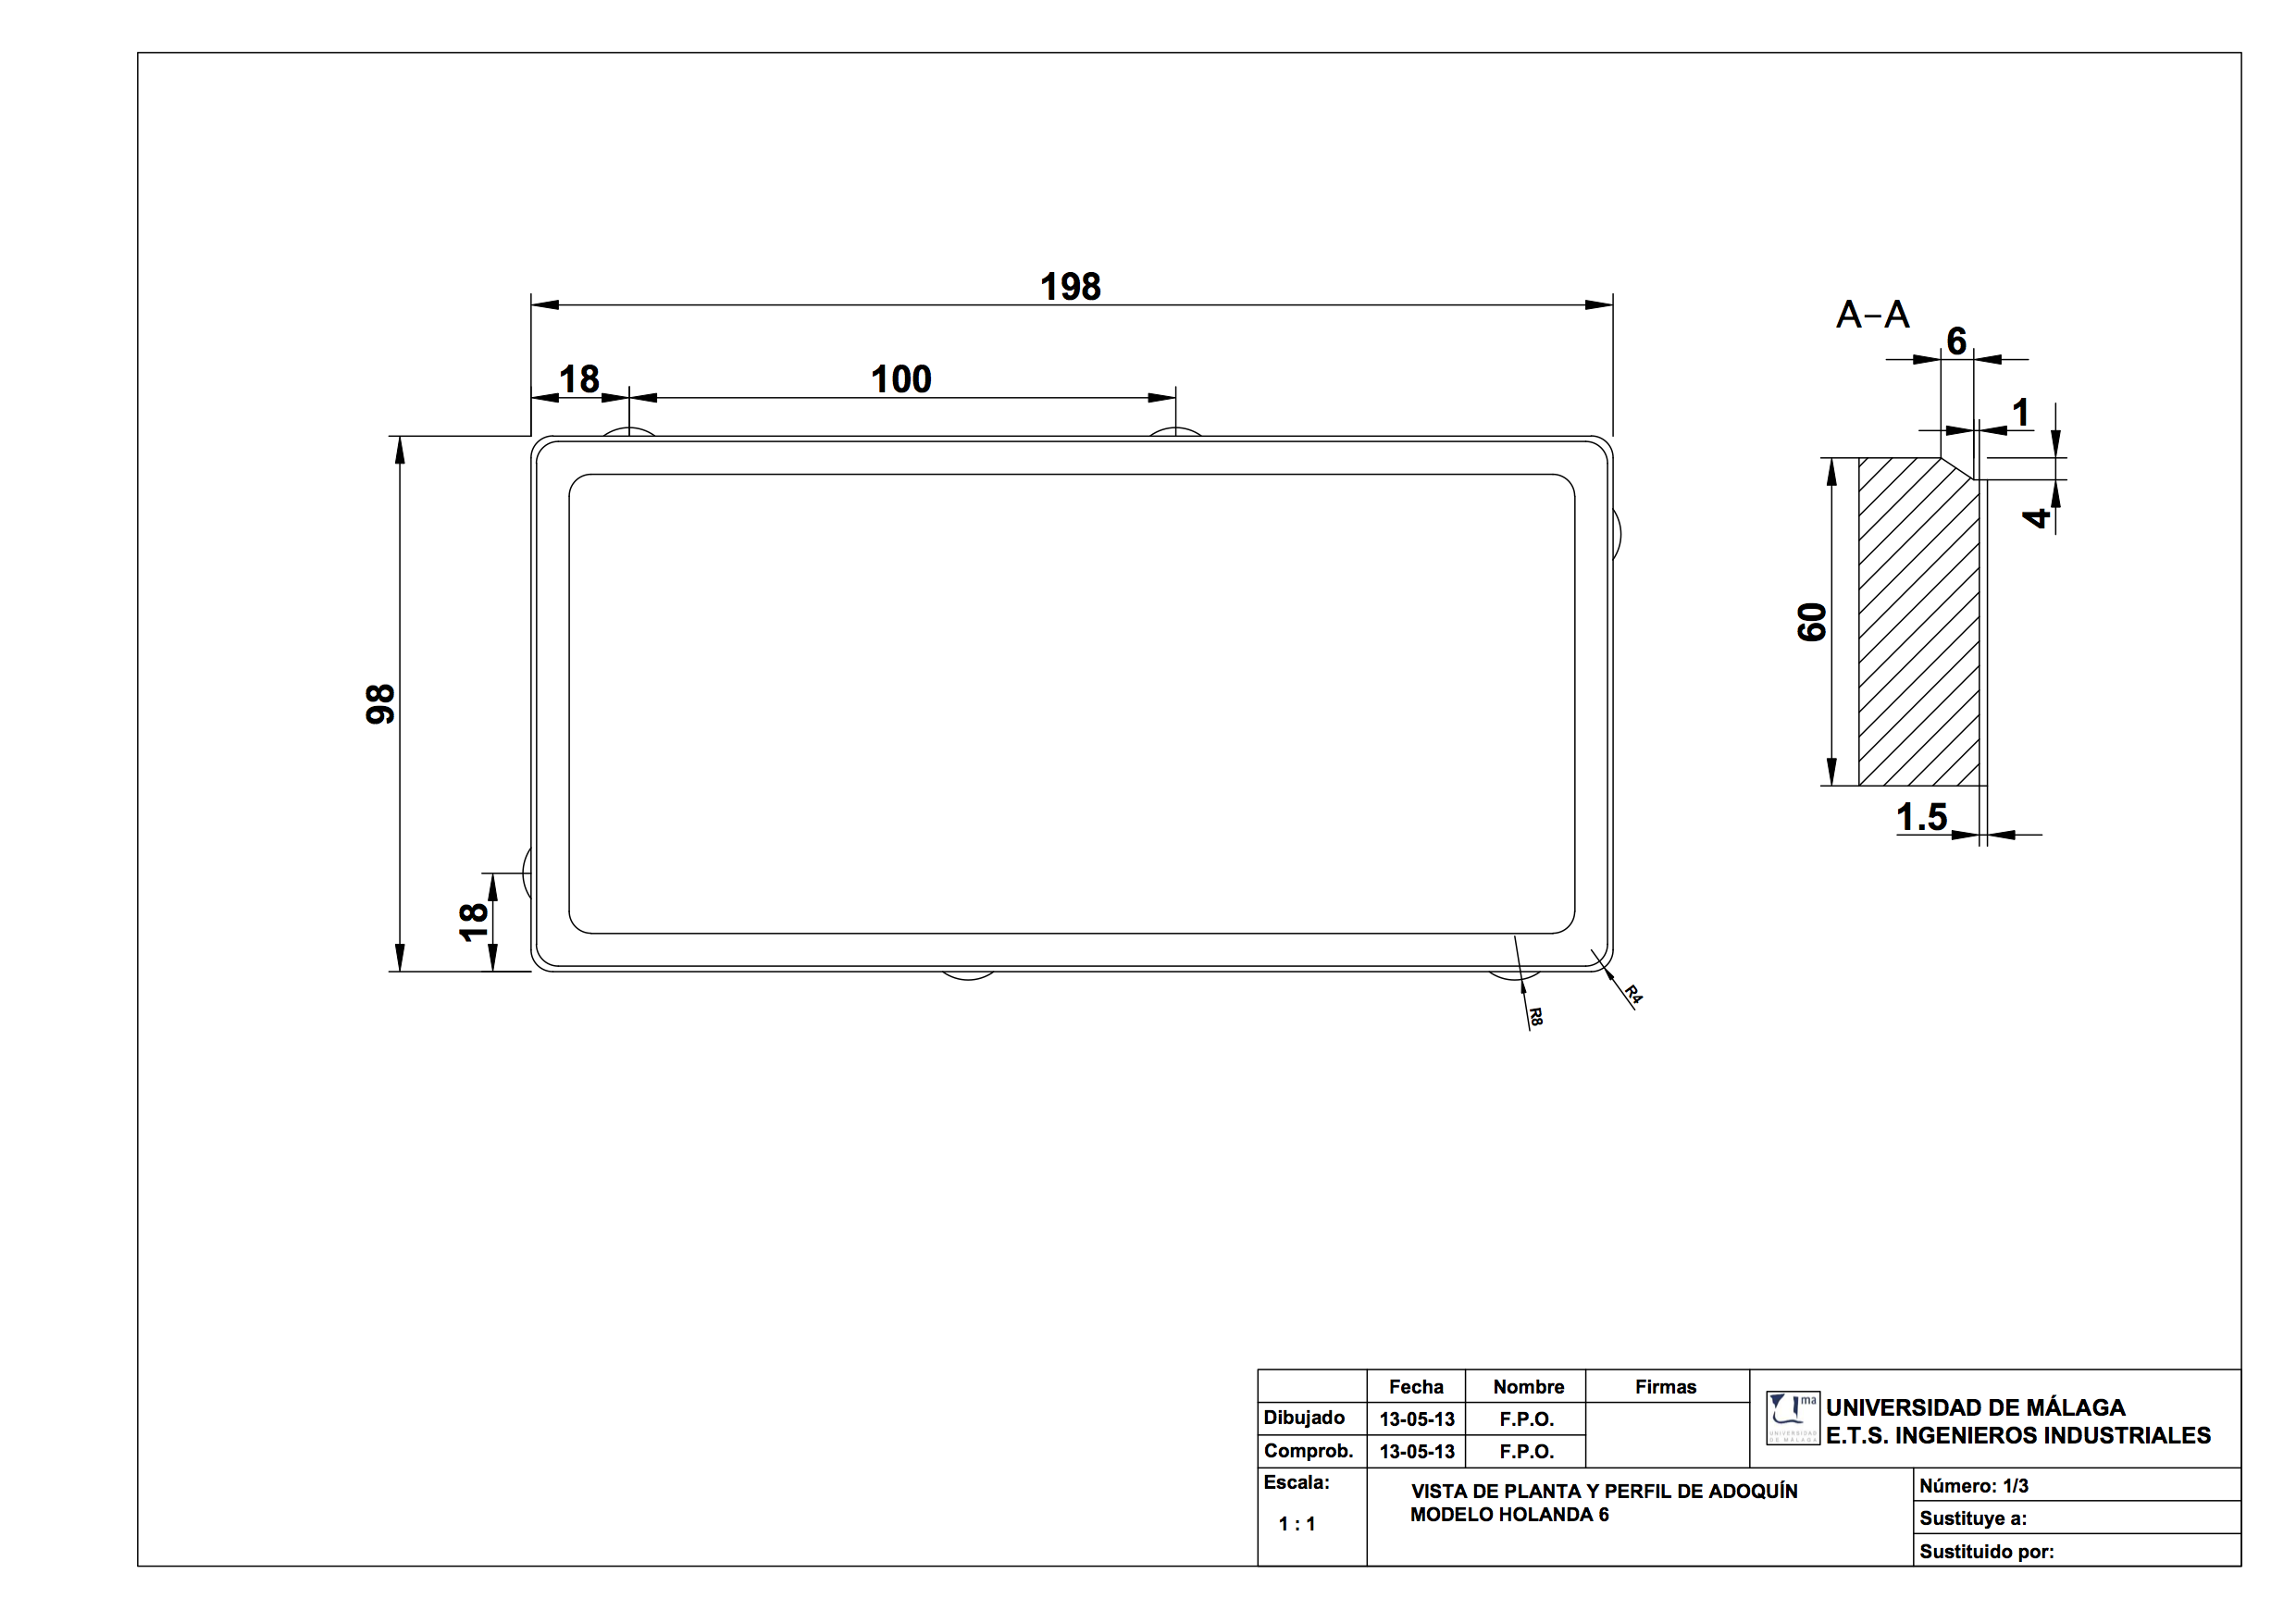
\includegraphics[angle=90,width=13.5cm]{plano_adoquin.png}
\end{figure}

\newpage
\setcounter{chapter}{2}
\addcontentsline{toc}{chapter}{\protect\numberline{\thechapter}Plano molde adoquín Holanda 6}
\begin{figure}[!htb]
\centering
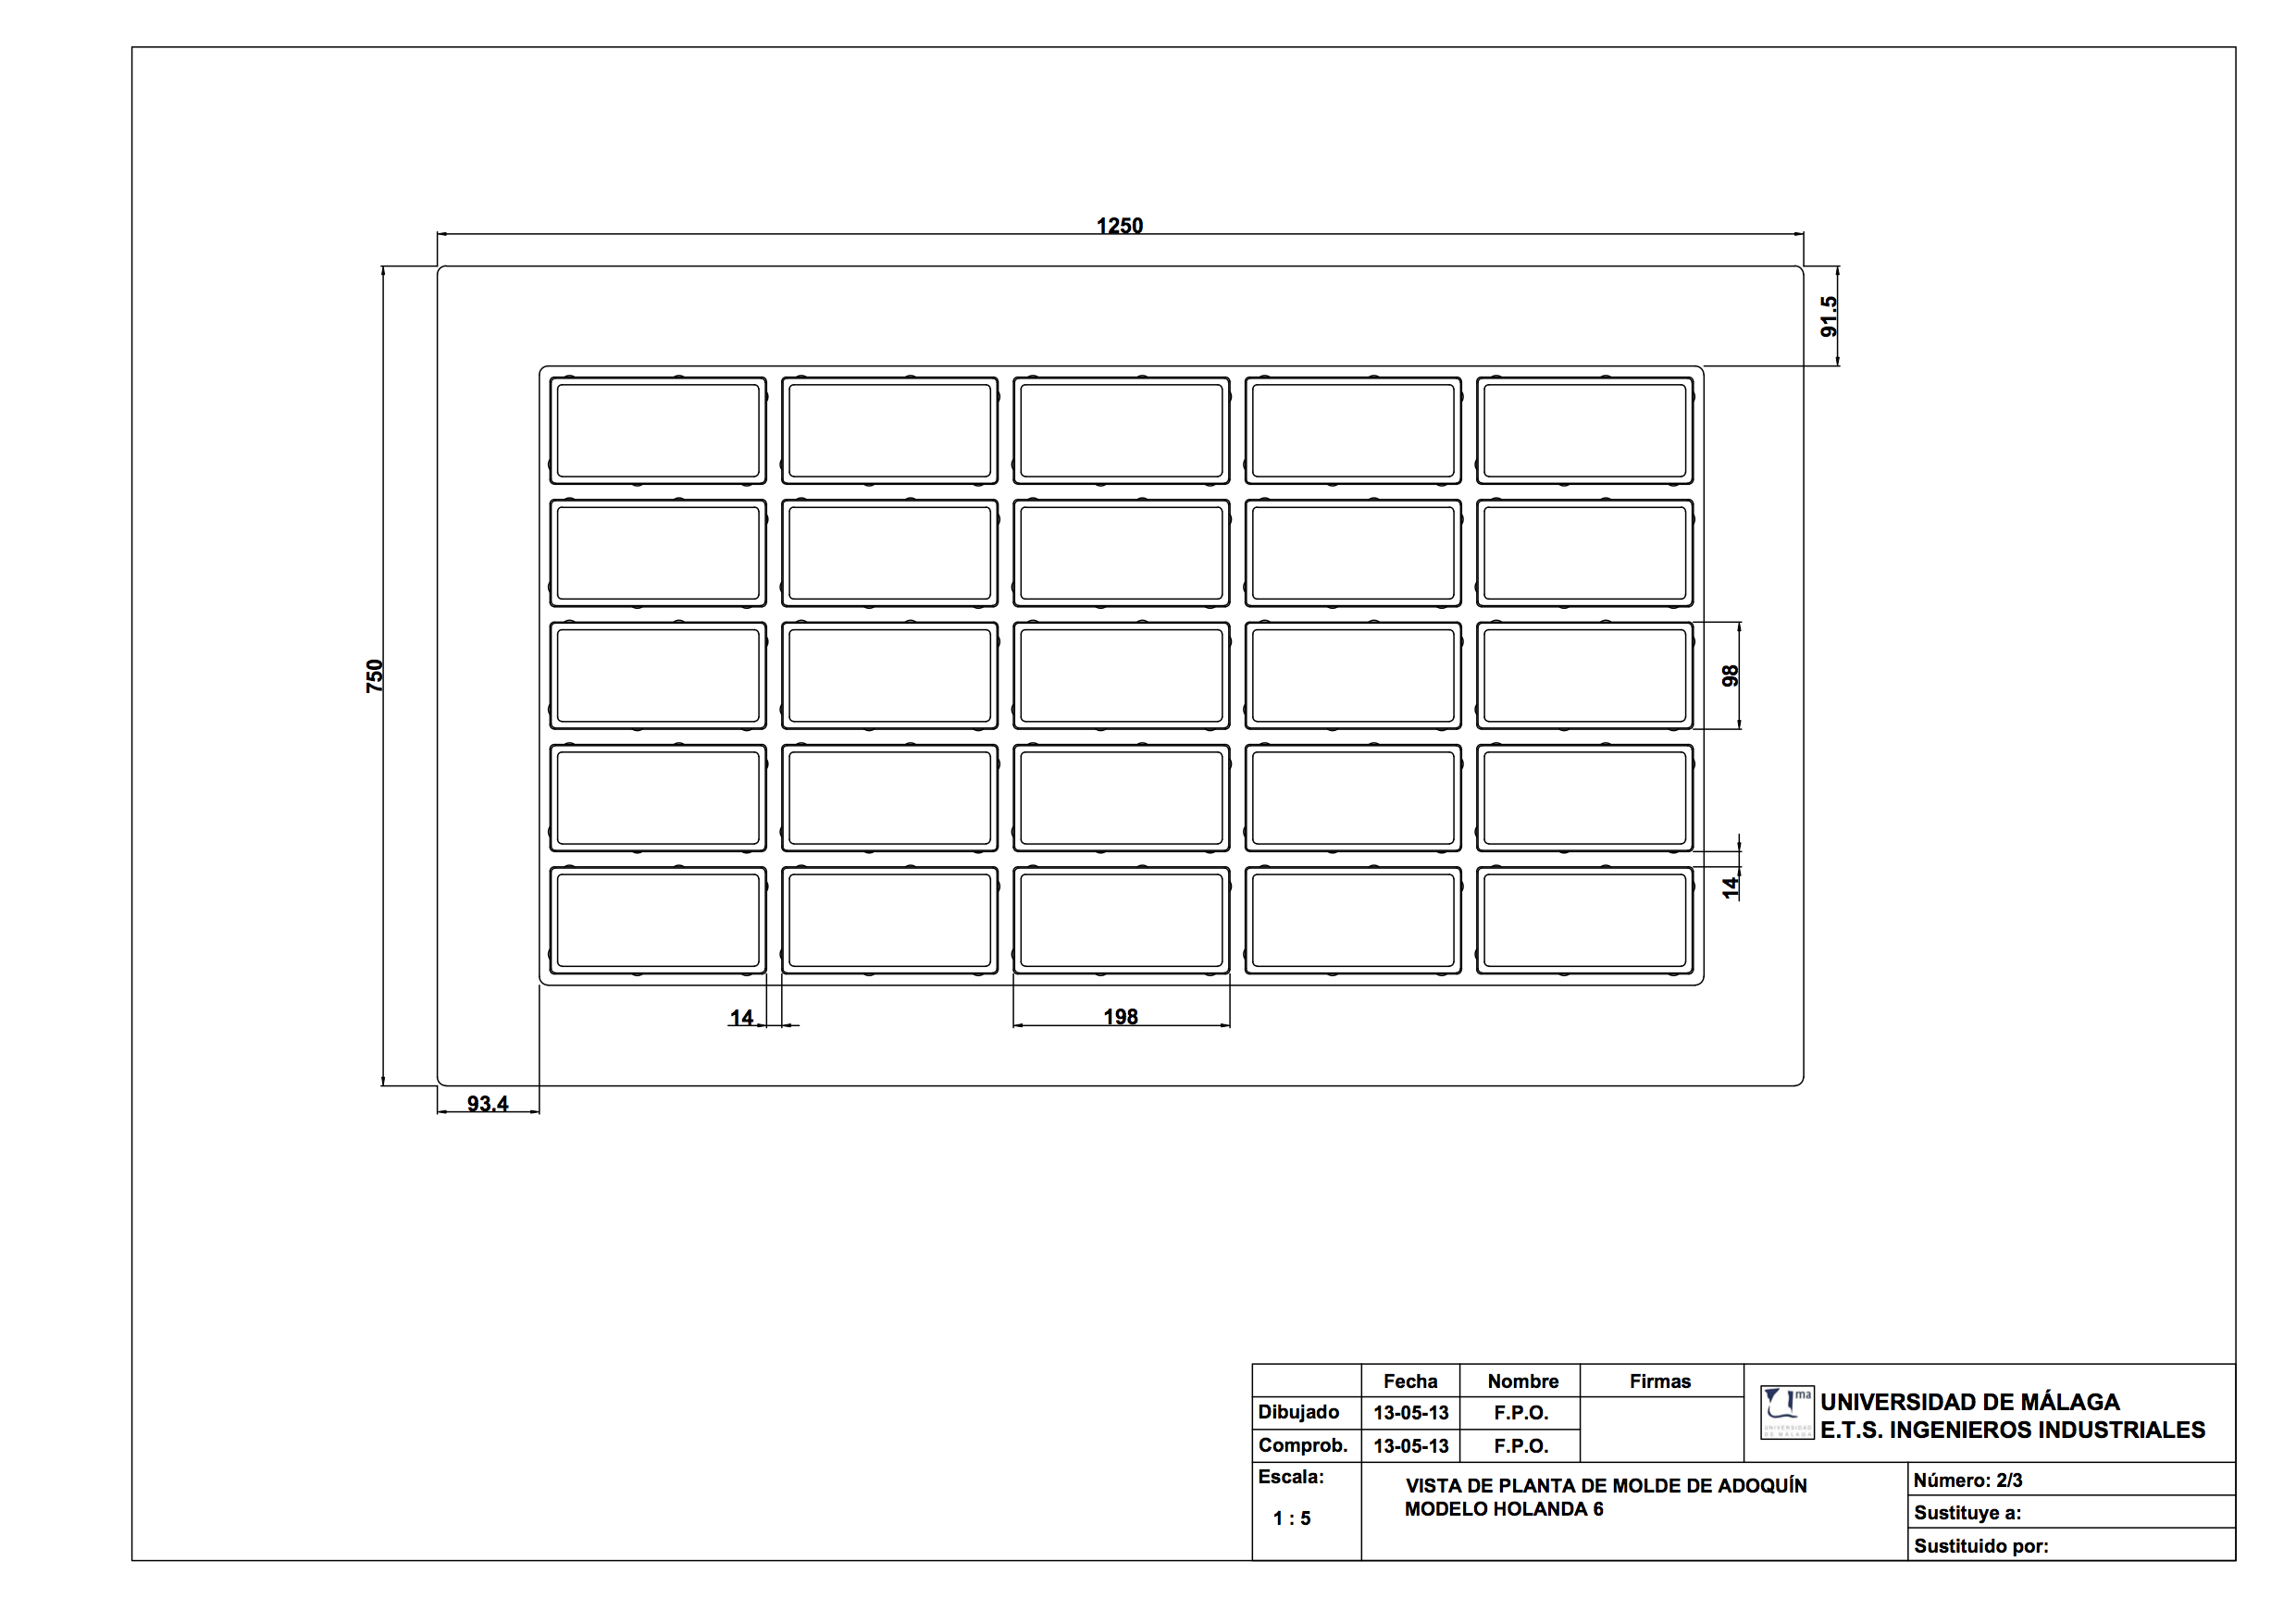
\includegraphics[angle=90,width=13.5cm]{plano_molde.png}
\end{figure}

\newpage
\setcounter{chapter}{3}
\addcontentsline{toc}{chapter}{\protect\numberline{\thechapter}Plano de instalaciones}
\begin{figure}[!htb]
\centering
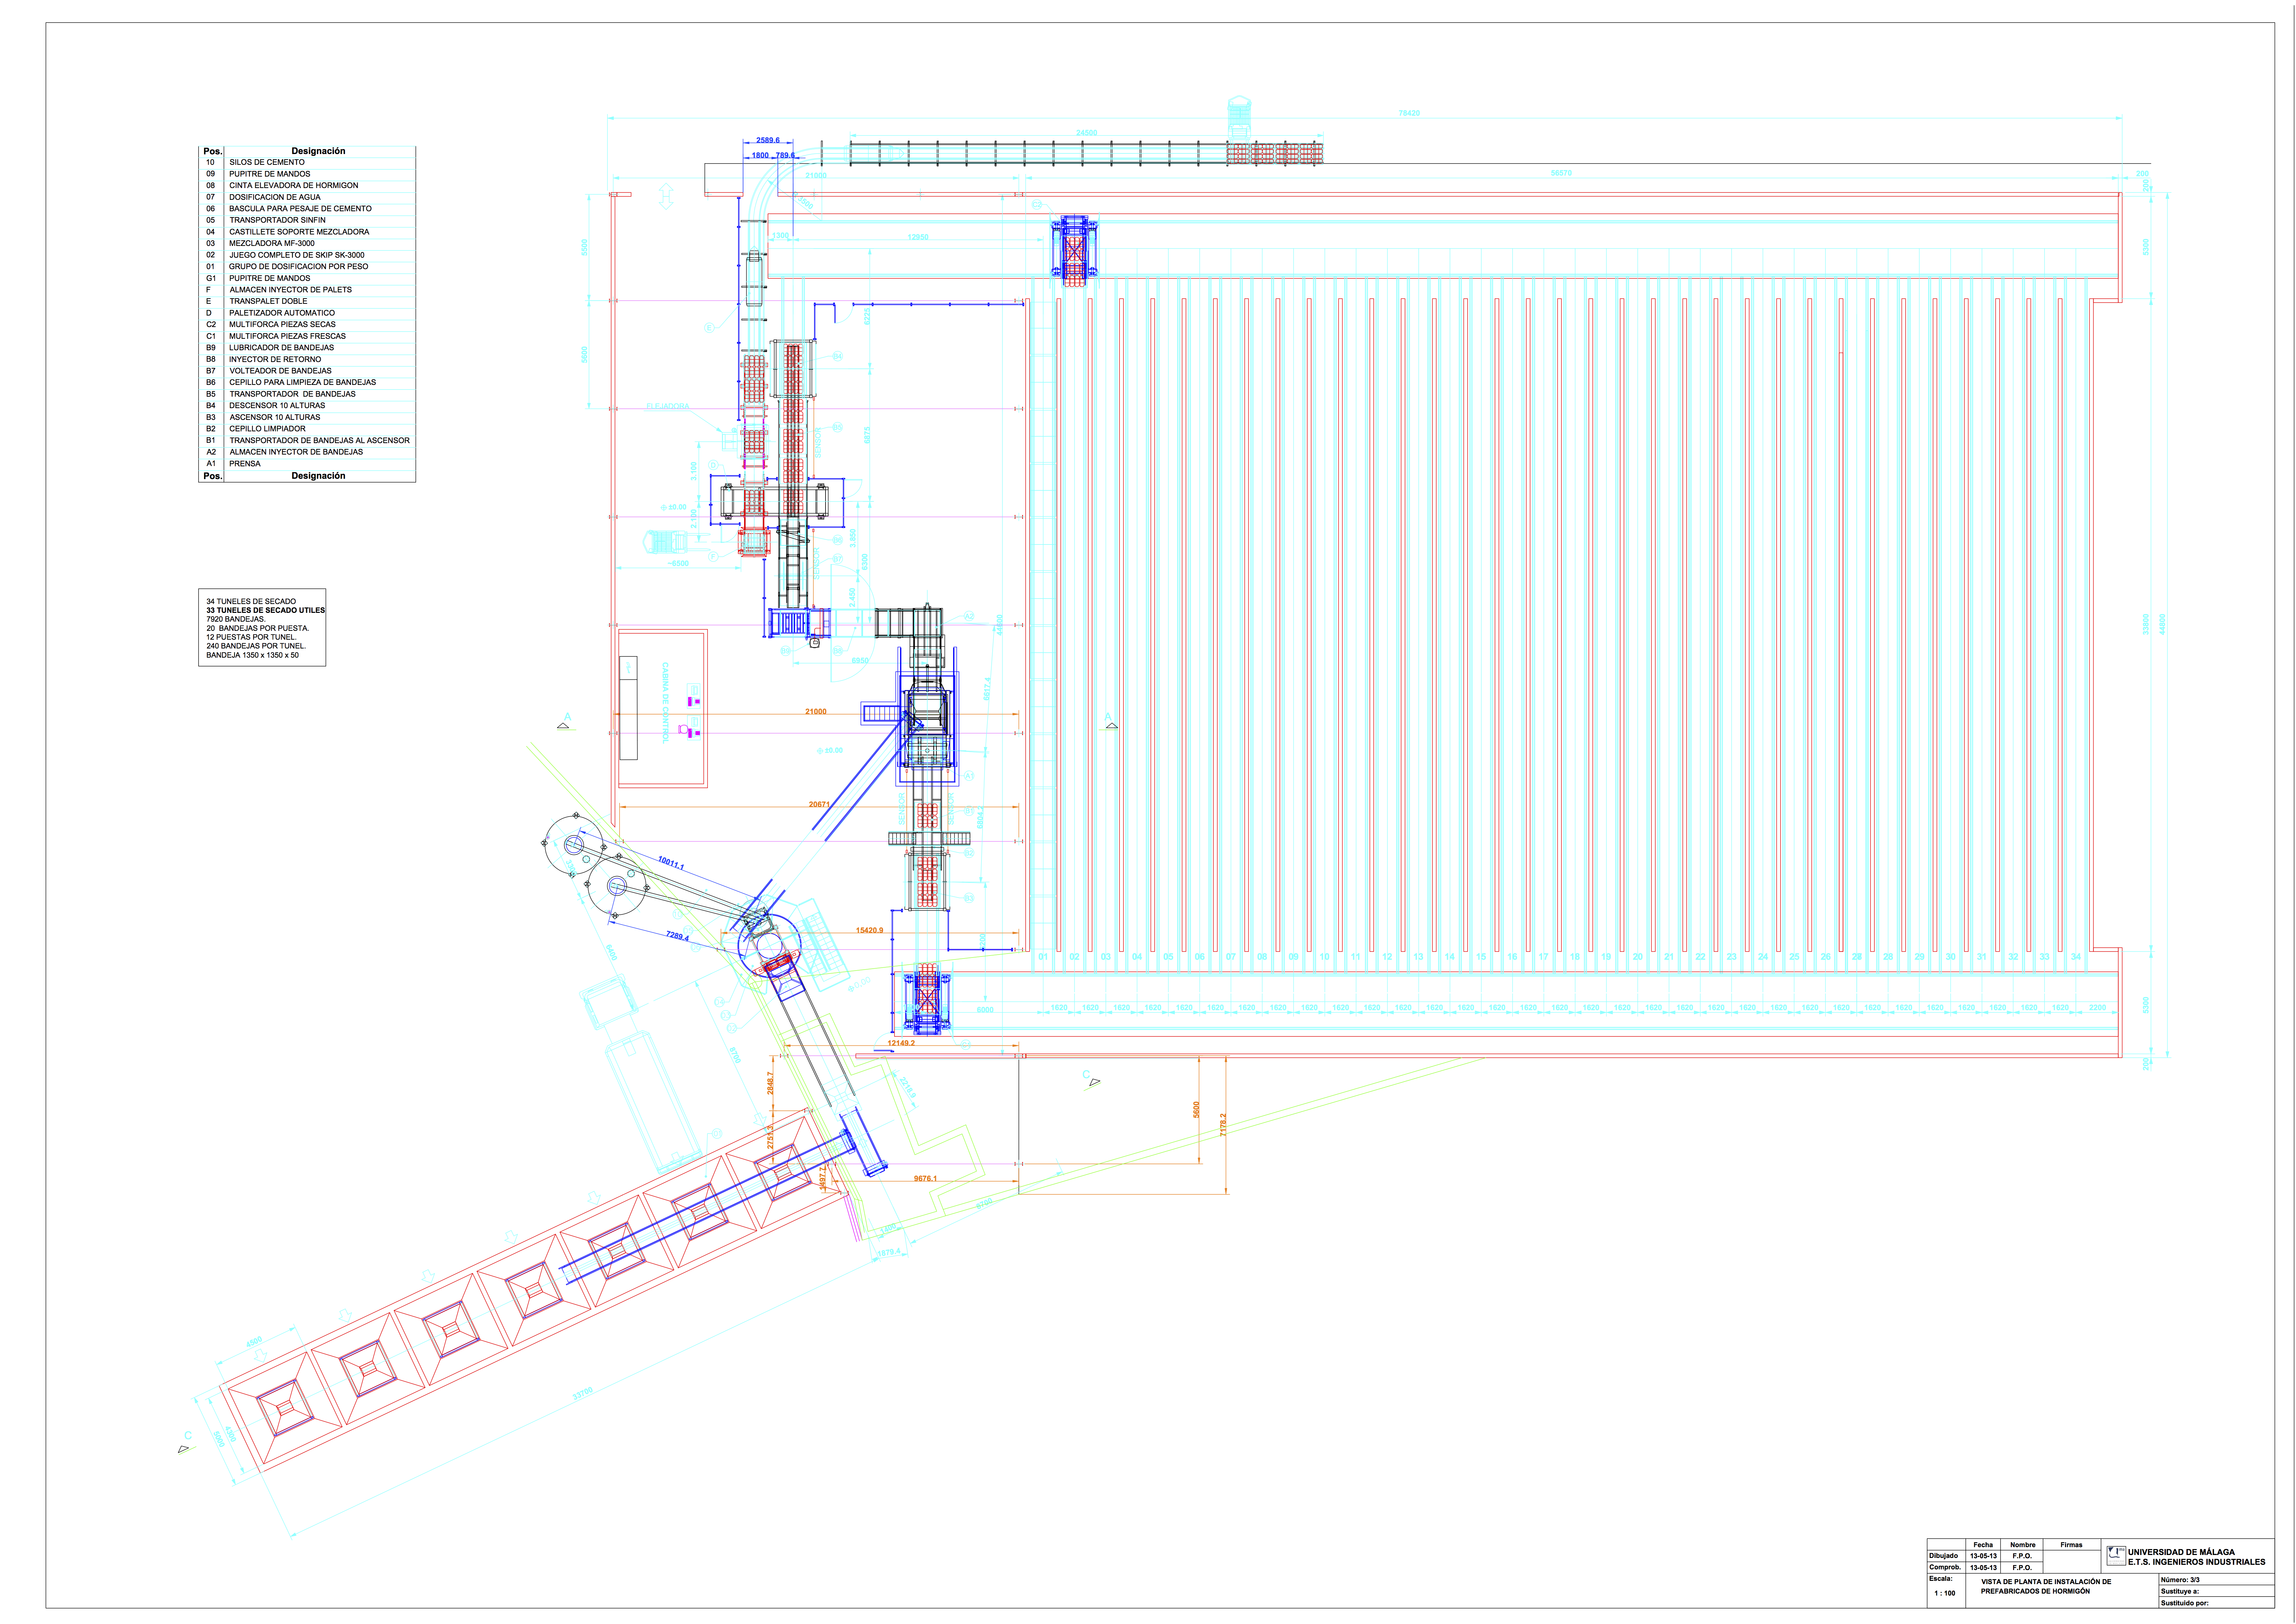
\includegraphics[angle=90,width=13.5cm]{plano_nave.png}
\end{figure}
